\documentclass[12pt]{article}
\usepackage[left=1cm, right=1cm, top=2cm,bottom=1.5cm]{geometry} 

\usepackage[parfill]{parskip}
\usepackage[utf8]{inputenc}
\usepackage[T2A]{fontenc}
\usepackage[russian]{babel}
\usepackage{enumitem}
\usepackage[normalem]{ulem}
\usepackage{amsfonts, amsmath, amsthm, amssymb, mathtools,xcolor}
\usepackage{blkarray}

\usepackage{tabularx}
\usepackage{hhline}

\usepackage{accents}
\usepackage{fancyhdr}
\pagestyle{fancy}
\renewcommand{\headrulewidth}{1.5pt}
\renewcommand{\footrulewidth}{1pt}

\usepackage{graphicx}
\usepackage[figurename=Рис.]{caption}
\usepackage{subcaption}
\usepackage{float}

%%Наименование папки откуда забирать изображения
\graphicspath{ {./images/} }

%%Изменение формата для ввода доказательства
\renewcommand{\proofname}{$\square$  \nopunct}
\renewcommand\qedsymbol{$\blacksquare$}

%%Изменение отступа на таблицах
\addto\captionsrussian{%
	\renewcommand{\proofname}{$\square$ \nopunct}%
}
%% Римские цифры
\newcommand{\RN}[1]{%
	\textup{\uppercase\expandafter{\romannumeral#1}}%
}

%% Для удобства записи
\newcommand{\MR}{\mathbb{R}}
\newcommand{\MC}{\mathbb{C}}
\newcommand{\MQ}{\mathbb{Q}}
\newcommand{\MN}{\mathbb{N}}
\newcommand{\MZ}{\mathbb{Z}}
\newcommand{\MTB}{\mathbb{T}}
\newcommand{\MTI}{\mathbb{I}}
\newcommand{\MI}{\mathrm{I}}
\newcommand{\MCI}{\mathcal{I}}
\newcommand{\MJ}{\mathrm{J}}
\newcommand{\MH}{\mathrm{H}}
\newcommand{\MT}{\mathrm{T}}
\newcommand{\MA}{\mathcal{A}}
\newcommand{\MCB}{\mathcal{B}}
\newcommand{\MCC}{\mathcal{C}}
\newcommand{\MU}{\mathcal{U}}
\newcommand{\MV}{\mathcal{V}}
\newcommand{\MB}{\mathcal{B}}
\newcommand{\MF}{\mathcal{F}}
\newcommand{\MW}{\mathcal{W}}
\newcommand{\ML}{\mathcal{L}}
\newcommand{\MP}{\mathcal{P}}
\newcommand{\VN}{\varnothing}
\newcommand{\VE}{\varepsilon}

\theoremstyle{definition}
\newtheorem{defn}{Опр:}
\newtheorem{rem}{Rm:}
\newtheorem{prop}{Утв.}
\newtheorem{exrc}{Упр.}
\newtheorem{problem}{Задача}
\newtheorem{lemma}{Лемма}
\newtheorem{theorem}{Теорема}
\newtheorem{corollary}{Следствие}

\newenvironment{cusdefn}[1]
{\renewcommand\thedefn{#1}\defn}
{\enddefn}

\DeclareRobustCommand{\divby}{%
	\mathrel{\text{\vbox{\baselineskip.65ex\lineskiplimit0pt\hbox{.}\hbox{.}\hbox{.}}}}%
}
%Короткий минус
\DeclareMathSymbol{\SMN}{\mathbin}{AMSa}{"39}
%Длинная шапка
\newcommand{\overbar}[1]{\mkern 1.5mu\overline{\mkern-1.5mu#1\mkern-1.5mu}\mkern 1.5mu}
%Функция знака
\DeclareMathOperator{\sgn}{sgn}

%Функция ранга
\DeclareMathOperator{\rk}{\text{rk}}
\DeclareMathOperator{\diam}{\text{diam}}


%Обозначение константы
\DeclareMathOperator{\const}{\text{const}}

\DeclareMathOperator{\codim}{\text{codim}}

\DeclareMathOperator*{\dsum}{\displaystyle\sum}
\newcommand{\ddsum}[2]{\displaystyle\sum\limits_{#1}^{#2}}

%Интеграл в большом формате
\DeclareMathOperator{\dint}{\displaystyle\int}
\newcommand{\ddint}[2]{\displaystyle\int\limits_{#1}^{#2}}
\newcommand{\ssum}[1]{\displaystyle \sum\limits_{n=1}^{\infty}{#1}_n}

\newcommand{\smallerrel}[1]{\mathrel{\mathpalette\smallerrelaux{#1}}}
\newcommand{\smallerrelaux}[2]{\raisebox{.1ex}{\scalebox{.75}{$#1#2$}}}

\newcommand{\smallin}{\smallerrel{\in}}
\newcommand{\smallnotin}{\smallerrel{\notin}}

\newcommand*{\medcap}{\mathbin{\scalebox{1.25}{\ensuremath{\cap}}}}%
\newcommand*{\medcup}{\mathbin{\scalebox{1.25}{\ensuremath{\cup}}}}%

\makeatletter
\newcommand{\vast}{\bBigg@{3.5}}
\newcommand{\Vast}{\bBigg@{5}}
\makeatother

%Промежуточное значение для sup\inf, поскольку они имеют разную высоту
\newcommand{\newsup}{\mathop{\smash{\mathrm{sup}}}}
\newcommand{\newinf}{\mathop{\mathrm{inf}\vphantom{\mathrm{sup}}}}

%Скалярное произведение
\newcommand{\inner}[2]{\left\langle #1, #2 \right\rangle }
\newcommand{\linsp}[1]{\left\langle #1 \right\rangle }
\newcommand{\linmer}[2]{\left\langle #1 \vert #2\right\rangle }

%Подпись символов снизу
\newcommand{\ubar}[1]{\underaccent{\bar}{#1}}

%% Шапка для букв сверху
\newcommand{\wte}[1]{\widetilde{#1}}
\newcommand{\wht}[1]{\widehat{#1}}

%%Трансформация Фурье
\newcommand{\fourt}[1]{\mathcal{F}\left(#1\right)}
\newcommand{\ifourt}[1]{\mathcal{F}^{-1}\left(#1\right)}

%%Символ вектора
\newcommand{\vecm}[1]{\overrightarrow{#1\,}}

%%Пространстов матриц
\newcommand{\mat}[2]{\operatorname{Mat}_{#1, #2}}


%%Взятие в скобки, модули и норму
\newcommand{\parfit}[1]{\left( #1 \right)}
\newcommand{\modfit}[1]{\left| #1 \right|}
\newcommand{\sqparfit}[1]{\left\{ #1 \right\}}
\newcommand{\normfit}[1]{\left\| #1 \right\|}

%%Функция для обозначения равномерной сходимости по множеству
\newcommand{\uconv}[1]{\overset{#1}{\rightrightarrows}}
\newcommand{\uconvm}[2]{\overset{#1}{\underset{#2}{\rightrightarrows}}}


%%Функция для обозначения нижнего и верхнего интегралов
\def\upint{\mathchoice%
	{\mkern13mu\overline{\vphantom{\intop}\mkern7mu}\mkern-20mu}%
	{\mkern7mu\overline{\vphantom{\intop}\mkern7mu}\mkern-14mu}%
	{\mkern7mu\overline{\vphantom{\intop}\mkern7mu}\mkern-14mu}%
	{\mkern7mu\overline{\vphantom{\intop}\mkern7mu}\mkern-14mu}%
	\int}
\def\lowint{\mkern3mu\underline{\vphantom{\intop}\mkern7mu}\mkern-10mu\int}

%%След матрицы
\DeclareMathOperator*{\tr}{tr}

\makeatletter
\renewcommand*\env@matrix[1][*\c@MaxMatrixCols c]{%
	\hskip -\arraycolsep
	\let\@ifnextchar\new@ifnextchar
	\array{#1}}
\makeatother


%% Переопределение функции хи, чтобы выглядела более приятно
\makeatletter
\@ifdefinable\@latex@chi{\let\@latex@chi\chi}
\renewcommand*\chi{{\@latex@chi\smash[t]{\mathstrut}}} % want only bottom half of \mathstrut
\makeatletter

\begin{document}
\lhead{Алгебра-\RN{1}}
\chead{Тимашев Д.А.}
\rhead{Лекция - 5}
\section*{Линейные отображения}

\begin{defn}
	Пусть $V, W$ - векторные пространства. Отображение $\MA \colon V \to W$ называется \uwave{линейным}, если оно согласованно с операциями в этих пространствах:
	\begin{enumerate}[label=\arabic*)]
		\item $\forall x,y \in V, \, \MA(x + y) = \MA(x) + \MA(y)$;
		\item $\forall x \in V,\, \forall \lambda \in \MR, \, \MA(\lambda{\cdot}x) = \lambda{\cdot}\MA(x)$;
	\end{enumerate}
\end{defn}

\subsection*{Примеры линейных отображений}
\begin{enumerate}[label=(\arabic*)]
	\item $V = W = \{\text{геом. векторы на плоскости}\}$, $\MA$ - поворот на угол $\alpha$ относительно $0$.
	\begin{figure}[H]
		\centering
		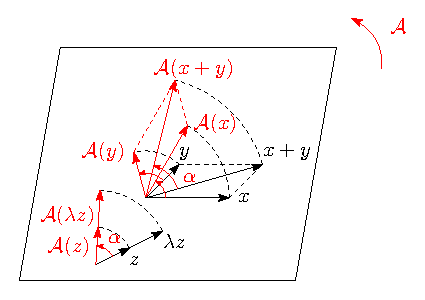
\includegraphics[width=0.3\textwidth]{AL1L5_1.eps}
		\caption{Поворот в геометрическом пространстве.}
		\label{5_1}
	\end{figure}
	\begin{proof} Оба свойства линейного отображения очевидно выполнены:
		\begin{enumerate}[label=\arabic*)]
			\item после поворота длина векторов не меняется, угол между векторами сохраняется $\Rightarrow$ параллелограмм переходит в параллелограмм;
			\item растяжение вектора переходит в то же растяжение, только после поворота;
		\end{enumerate}
		Можно это же показать, используя матричный подход (см. матрицу поворота).
	\end{proof}

	\item $V = \{\text{геом. векторы в пространстве}\}$, $W = \{\text{геом. векторы на плоскости } P \text{ в пространстве}\}$ и рассмотрим $\MA$ - проекцию на плоскость $P$.
	\begin{figure}[H]
		\centering
		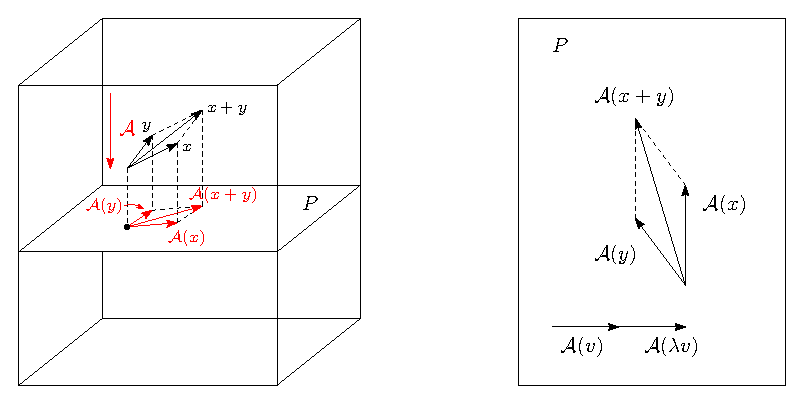
\includegraphics[width=0.7\textwidth]{AL1L5_2.eps}
		\caption{Проекция вектора на плоскость.}
		\label{5_2}
	\end{figure}
	\begin{proof}
		Оба свойства линейного отображения выполнены:
		\begin{enumerate}[label=\arabic*)]
			\item проекция суммы двух векторов будет равна сумме проекций, поскольку векторы проектируются параллельно прямой $\Rightarrow$ начала и концы векторов на плоскости будут проектироваться однозначно $\Rightarrow$ параллелограмм проектируется в параллелограмм;
			\item растяжение векторов дает такое же увеличение их проекций;
		\end{enumerate}
		Можно это же показать, используя матричный подход (см. проекторы).
	\end{proof}
\end{enumerate}

\subsection*{Линейные отображения арифметических пространств}
Далее будем рассматривать только линейные отображения арифметических пространств $\MR^n \to \MR^m$. Будем интерпретировать арифметические пространства, как пространства столбцов.
\begin{rem}
	Заметим, что любое конечномерное пространство можно отождествить с арифметическим пространством: выбрать базис и тогда каждый вектор будет задаваться столбцом своих координат.
\end{rem}
Оказывается, что линейные отображения арифметических пространств можно задавать с помощью матриц.
\begin{defn}
	\uwave{Матрицей линейного отображения} $\MR^n \to \MR^m$ называется матрица $A$ размера $m \times n$, столбцы которой определяются следующим образом:
	$$
		A^{(j)} = \MA(e_j), \, \forall j = \overline{1,n}
	$$
	где $(e_1, \dotsc, e_n)$ - стандартный базис в $\MR^n$, то есть $A = \left(\MA(e_1),\dotsc, \MA(e_j),\dotsc \MA(e_n)\right)$.
\end{defn}

\uline{\textbf{Соглашение по обозначениям}}: линейные отображение - заглавные рукописные латинские буквы, а их матрицы - заглавные печатные латинские буквы.
\begin{prop}
	Линейное отображение $\MA$ однозначно определяется своей матрицей $A$.
\end{prop}
\begin{proof}
	Матрица показывает каковы образы базисных векторов, но если мы знаем образы базисных векторов, то мы можем посчитать образ любого вектора. В самом деле:
	$$
		\forall x \in \MR^n, \, x = x_1{\cdot} e_1 + \dotsc + x_n{\cdot} e_n \Rightarrow x = \begin{pmatrix}
			x_1 \\
			\vdots\\
			x_i\\
			\vdots\\
			x_n
		\end{pmatrix} \Rightarrow 
	$$
	$$
		\Rightarrow \MA(x) = \MA(x_1 {\cdot}e_1) + \dotsc + \MA(x_n{\cdot} e_n)  = x_1{\cdot}\MA(e_1) + \dotsc + x_n {\cdot}\MA(e_n) = A^{(1)}{\cdot}x_1 + \dotsc + A^{(n)}{\cdot}x_n
	$$
	где мы воспользовались свойствами линейного отображения. То есть мы получили линейную комбинацию столбцов матрицы $A$ с коэффициентами, которые равны координатам вектора $x \Rightarrow$ зная матрицу можно написать образ любого вектора $\Rightarrow$ линейное отображение однозначно задается матрицей. Заметим, что это по сути тоже самое, что и инъективность отображения из множества линейных отображений в множество матриц:
	$$
		\forall i = \overline{1,n}, \, \MA(e_i) = \MCB(e_i) \Rightarrow A^{(i)} = B^{(i)} \Rightarrow \forall x \in \MR^n, \, \MA(x) = \MCB(x) 
	$$
\end{proof}

\begin{prop}
	Любая матрица $A$ размера $m\times n$ определяет линейное отображение $\MA\colon \MR^n \to \MR^m$ по формуле:
	$$
		\MA(x) = A^{(1)}{\cdot}x_1 + \dotsc + A^{(n)}{\cdot}x_n
	$$
\end{prop}
\begin{proof}
	По формуле мы определяем образ вектора $x \in \MR^n$ как линейную комбинацию столбцов матрицы $A$ с коэффициентами, которые равны координатам вектора $x$. Легко видеть, что эта формула задает линейное отображение:
	\begin{enumerate}[label=\arabic*)]
		\item $\forall x,y \in \MR^n$:
		$$
			\MA(x + y) = A^{(1)}(x_1 + y_1) + \dotsc + A^{(n)}(x_n + y_n) = A^{(1)}{\cdot}x_1 + \dotsc + A^{(n)}{\cdot}x_n +
		$$
		$$
			+ A^{(1)}{\cdot}y_1 + \dotsc + A^{(n)}{\cdot}y_n = \MA(x) + \MA(y)
		$$
		\item $\forall x \in \MR^n,\, \forall \lambda \in \MR, \, \MA(\lambda{\cdot}x) = A^{(1)}{\cdot}(\lambda{\cdot}x_1) + \dotsc + A^{(n)}{\cdot}(\lambda{\cdot}x_n) = \lambda{\cdot}(A^{(1)}{\cdot}x_1 + \dotsc + A^{(n)}{\cdot}x_n) = \lambda{\cdot}\MA(x)$;
	\end{enumerate}
	По сути, это тоже самое, что и сюръективность отображения из множества линейных отображений в множество матриц.
\end{proof}
\begin{corollary}
	Между множеством линейных отображений $\MR^n \to \MR^m$ и множеством матриц размера $m\times n$ существует взаимнооднозначное соответствие:
	$$
		 \{\text{линейные отображения: } \MR^n \to \MR^m\} \leftrightarrow \mat{m}{n}
	$$
\end{corollary}

\subsection*{Интерпритация СЛУ на языке линейных отображений}
Пусть у нас есть произвольная СЛУ с матрицей коэффициентов $A$:
$$
	\left\{
	\begin{array}{ccccccccccc}
		a_{11}x_1 & + & \dotsc & + & a_{1j}x_j & + & \dotsc & + & a_{1n}x_n & = & b_1 \\
		a_{21}x_1 & + & \dotsc & + & a_{2j}x_j & + & \dotsc & + & a_{2n}x_n & = & b_2 \\
		\vdots & \vdots &\ddots & \vdots & \vdots & \vdots & \ddots & \vdots & \vdots & \vdots & \vdots \\ 
		a_{m1}x_1 & + & \dotsc & + & a_{mj}x_j & + & \dotsc & + & a_{mn}x_n & = & b_m 
	\end{array}
	\right., \quad
	A = 
	\begin{pmatrix}
		a_{11} & \dotsc & a_{1j} & \dotsc & a_{1n}\\
		\vdots & \ddots & \vdots & \ddots & \vdots \\
		a_{m1} & \dotsc & a_{mj} & \dotsc & a_{mn}
	\end{pmatrix}, \, 
	b = 
	\begin{pmatrix}
		b_1 \\
		\vdots \\
		b_m
	\end{pmatrix}
$$
Матрица $\underset{m \times n}{A} \in \mat{m}{n}$ - матрица коэффициентов СЛУ и столбец $\underset{m \times 1}{b} \in \MR^m$ - столбец свободных членов. Вектор-столбец $x^{\circ} \in \MR^n$ является решением СЛУ $\Leftrightarrow$ при подстановке вместо неизвестных значений, мы получим верные равенства, то есть если мы сложим столбцы матрицы $A$ с коэффициентами равными координатам $x^{\circ}$, то мы получим столбец $b$:
$$
	A^{(1)}{\cdot}x_1^{\circ}+ \dotsc + A^{(j)} {\cdot}x_j^{\circ} + \dotsc + A^{(n)}{\cdot}x_n^{\circ} = b \Leftrightarrow \MA(x^{\circ}) = b
$$
где $\MA \colon \MR^n \to \MR^m$ - линейное отображение, соответствующее матрице $A$.

\uline{\textbf{Множество решений СЛУ}}: это множество тех векторов, которые отображатся в $b$ при линейном отображении $\MA$, то есть это: $\MA^{-1}(b)$ - полный прообраз вектора $b$ при отображении $A$.

\subsection*{Алгебраические операции над линейными отображениями и матрицами}
Операции над линейными отображениями можно определять и исследовать на языке линейных отображений, а можно на языке матриц, поскольку есть взаимнооднозначное соответствие между отображениями и матрицами. Мы будем изначально давать определения для линейных отображений (поскольку это проще), а затем смотреть во что это превращается для матриц.

\begin{enumerate}[label=(\arabic*)]
	\item \uline{\textbf{Сложение}}:
	
	\textbf{Линейные отображения}: $\MA, \mathcal{B} \colon \MR^n \to \MR^m \Rightarrow \mathcal{C} = \MA +\mathcal{B} \colon \MR^n \to \MR^m$: 
	$$
		\mathcal{C}(x) = \MA(x) + \mathcal{B}(x), \, \forall x \in \MR
	$$ 
	
	\textbf{Матрицы}: $A,B \in \mat{m}{n} \Rightarrow C = A +B\in \mat{m}{n}$:
	$$
		C^{(j)} = \mathcal{C}(e_j) = \MA(e_j) + \mathcal{B}(e_j) = A^{(j)} + B^{(j)} \Rightarrow c_{ij} = a_{ij} + b_{ij}, \, \forall i = \overline{1,m}, j = \overline{1,n}
	$$
	\item \uline{\textbf{Умножение на число}}:
	
	\textbf{Линейные отображения}: $\MA \colon \MR^n \to \MR^m \Rightarrow \mathcal{C} = \lambda{\cdot}\MA \colon \MR^n \to \MR^m$:
	$$
		\mathcal{C}(x) = \lambda{\cdot}\MA(x), \, \forall x \in \MR^n
	$$
	
	\textbf{Матрицы}: $A\in \mat{m}{n} \Rightarrow C = \lambda{\cdot}A\in \mat{m}{n}$:
	$$
		C^{(j)} = \mathcal{C}(e_j) = \lambda{\cdot}\MA(e_j) = \lambda{\cdot}A^{(j)} \Rightarrow c_{ij} = \lambda{\cdot}a_{ij}, \, \forall i = \overline{1,m}, j = \overline{1,n}
	$$
	
	\item \uline{\textbf{Умножение}}:
	
	\textbf{Линейные отображения}: $\MA  \colon \MR^n \to \MR^m, \, \mathcal{B}\colon \MR^p \to \MR^n \Rightarrow \mathcal{C} = \MA {\cdot}\mathcal{B} \colon \MR^p \to \MR^m$:
	$$
		\mathcal{C} = \MA\big(\mathcal{B}(x)\big), \, \forall x \in \MR^p
	$$ 
	\begin{figure}[H]
		\centering
		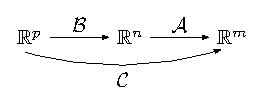
\includegraphics[width=0.25\textwidth]{AL1L5_3.eps}
		\caption{Композиция линейных отображений $\MA$ и $\mathcal{B}$.}
		\label{5_3}
	\end{figure}
	
	\textbf{Матрицы}: $A\in \mat{m}{n}$, $B\in \mat{n}{p}  \Rightarrow C = A{\cdot}B\in \mat{m}{p}$:
	$$
		C^{(j)} = \mathcal{C}(e'_j) = \MA \big(\mathcal{B}(e'_j) \big) = \MA\left(B^{(j)}\right) = \MA(b_{1j}{\cdot}e_1 + \dotsc +  b_{nj}{\cdot}e_n) = 
	$$
	$$
		=\MA(e_1){\cdot}b_{1j} + \MA(e_2){\cdot}b_{2j} + \dotsc + \MA(e_n){\cdot}b_{nj} = A^{(1)}{\cdot}b_{1j} + A^{(2)}{\cdot}b_{2j}+ \dotsc + A^{(n)}{\cdot}b_{nj} \Rightarrow
	$$
	$$
		\Rightarrow c_{ij} = a_{i1}b_{1j} + a_{i2}b_{2j} + \dotsc + a_{in}b_{nj} = \ddsum{k = 1}{n}a_{ik}{\cdot}b_{ij} , \, \forall i = \overline{1,m}, j = \overline{1,n}
	$$
	то есть это умножение строки на столбец;
\end{enumerate}

\textbf{Пример}: Рассмотрим перемножение матриц размера $2\times 3$ и $3 \times 2$:
$$
	\begin{pmatrix}
		1 & 2 & 3\\
		6 & 5 & 4
	\end{pmatrix} {\cdot}
	\begin{pmatrix}
		-1 & 0 \\
		0 & 1 \\
		1 & -1
	\end{pmatrix} =
	\begin{pmatrix}
		1{\cdot}(-1) + 2{\cdot}0 + 3{\cdot}1 & 1{\cdot}0 + 2{\cdot}1 + 3{\cdot}(-1)\\
		6{\cdot}(-1) + 5{\cdot}0 + 4{\cdot}1 & 6{\cdot}0 + 5{\cdot}1 + 4{\cdot}(-1)\\
	\end{pmatrix} = 
	\begin{pmatrix}
		2 & -1 \\
		-2 & 1
	\end{pmatrix}
$$
\begin{prop}(\textbf{проверка корректности определения операций над линейными отображениями})
	Операции заданные над линейными отображениями - корректны.
\end{prop}
\begin{proof}
	Проверим, что все полученные отображения - линейные.
	\begin{enumerate}[label=(\arabic*)]
		\item \uline{\textbf{Сложение}}: $\MCC = \MA + \MCB$
			\begin{enumerate}[label=\arabic*)]
				\item $\forall x,y \in \MR^n, \, \MCC(x + y) = \MA(x+y) + \MCB(x+y) = \MA(x) + \MA(y) + \MCB(x) + \MCB(y) = \MCC(x) + \MCC(y)$;
				\item $\forall x \in \MR^n, \, \forall \lambda \in \MR, \, \MCC(\lambda{\cdot}x) = \MA(\lambda{\cdot}x) + \MCB(\lambda{\cdot}y) = \lambda{\cdot}\MA(x) + \lambda{\cdot}\MCB(x) = \lambda{\cdot}(\MA(x)+ \MCB(x)) = \lambda{\cdot}\MCC(x)$;
			\end{enumerate}
		\item \uline{\textbf{Умножение на число}}: $\MCC = \mu{\cdot}\MA$
			\begin{enumerate}[label=\arabic*)]
				\item $\forall x,y \in \MR^n, \, \MCC(x + y) = \mu{\cdot}\MA(x +y) = \mu{\cdot}\MA(x) + \mu{\cdot}\MA(y) = \MCC(x) + \MCC(y)$;
				\item $\forall x \in \MR^n, \, \forall \lambda \in \MR, \, \MCC(\lambda{\cdot}x) = \mu{\cdot}\MA(\lambda{\cdot}x) = \lambda{\cdot}\mu{\cdot} \MA(x) = \lambda{\cdot}\MCC(x)$;
			\end{enumerate}
		\item \uline{\textbf{Умножение}}: $\MCC = \MA{\cdot}\MCB$
		\begin{enumerate}[label=\arabic*)]
			\item $\forall x,y \in \MR^n, \, \MCC(x + y) = \MA(\MB(x+y)) = \MA(\MB(x) + \MB(y)) =\MA(\MCB(x)) + \MA(\MCB(y)) = \MCC(x) + \MCC(y)$;
			\item $\forall x \in \MR^n, \, \forall \lambda \in \MR, \, \MCC(\lambda{\cdot}x) = \MA(\MCB(\lambda{\cdot}x)) = \MA(\lambda{\cdot}\MCB(x)) = \lambda{\cdot}\MA(\MB(x)) = \lambda{\cdot}\MCC(x)$;
		\end{enumerate}
	\end{enumerate}
\end{proof}

\subsection*{Матричная запись линейного отображения}

Пусть $\MA \colon \MR^n \to \MR^m$, хотим записать $\MA(x), \, x \in \MR^n$. Запишем в матричном виде:
$$
	x = 
	\begin{pmatrix}
		x_1 \\
		\vdots \\ 
		x_n
	\end{pmatrix} \in \MR^n, \, y = \MA(x) = 
	\begin{pmatrix}
		y_1 \\
		\vdots \\
		y_m
	\end{pmatrix} \in \MR^m 
$$
Распишем $y$ подробнее и рассмотрим $i$-ую координату:
$$
	y = \MA(x) = \MA(x_1 {\cdot}e_1 + \dotsc + x_n {\cdot}e_n) = A^{(1)}{\cdot}x_1 + A^{(2)}{\cdot}x_2+ \dotsc + A^{(n)}{\cdot}x_n \Rightarrow
$$
$$
	\Rightarrow y_i = a_{i1}x_1 + a_{i2}x_2 + \dotsc + a_{in}x_n = \begin{pmatrix}
		a_{i1},& a_{i2},& \dotsc \; ,& a_{in}
	\end{pmatrix}{\cdot}
	\begin{pmatrix}
		x_1 \\
		x_2 \\
		\vdots\\
		x_n
	\end{pmatrix}
$$
Запишем все эти равенства одно под другим, тогда мы получаем:
$$
	y = 	
	\begin{pmatrix}
		y_1 \\
		\vdots \\
		y_{i}\\
		\vdots\\
		y_m
	\end{pmatrix} = 
	\begin{pmatrix}
		a_{11} & \dotsc & a_{1n} \\
		\vdots & \ddots & \vdots \\
		a_{i1} & \dotsc & a_{in}\\
		\vdots & \ddots & \vdots \\
		a_{m1} & \dotsc & a_{mn}
	\end{pmatrix}{\cdot}
	\begin{pmatrix}
		x_1 \\
			\vdots \\
		x_i \\
		\vdots\\
		x_n
	\end{pmatrix} \Leftrightarrow y = A{\cdot}x
$$
Таким образом, получили формулу матричной записи линейного отображения: $y = A{\cdot}x$.

\subsection*{Матричная запись СЛУ}
Рассмотрим ту же систему, что мы рассматривали выше, где матрица коэффициентов $A$, столбец неизвестных $x$ и столбец свободных членов $b$:
$$
	A = 
	\begin{pmatrix}
		a_{11} & \dotsc & a_{1j} & \dotsc & a_{1n}\\
		\vdots & \ddots & \vdots & \ddots & \vdots \\
		a_{m1} & \dotsc & a_{mj} & \dotsc & a_{mn}
	\end{pmatrix}, \, 
	b = 
	\begin{pmatrix}
		b_1 \\
		\vdots \\
		b_m
	\end{pmatrix}, \, 
	x = 
	\begin{pmatrix}
		x_1\\
		\vdots \\
		x_n
	\end{pmatrix}
$$ 
На языке линейных отображений эта СЛУ записывается так: $\MA(x) = b \Rightarrow \MA(x) = A{\cdot}x = b$. 
\subsection*{Подстановка или замена переменных}
Подставим вместо $x_i$ другие переменные $y_j$, которые линейно выражаются через $x_i$:
$$
	\left\{
		\begin{array}{ccccccccc}
			x_1 & = & c_{11}y_1 & + & c_{12}y_2 & + & \dotsc & + & c_{1s}y_s\\
			x_2 & = & c_{21}y_1 & + & c_{22}y_2 & + & \dotsc & + & c_{2s}y_s\\
			\vdots & \vdots & \vdots & \vdots & \vdots & \vdots & \ddots & \vdots & \vdots\\
			x_n & = & c_{n1}y_1 & + & c_{n2}y_2 & + & \dotsc & + & c_{ns}y_s\\
		\end{array}
	\right.
$$
СЛУ тогда примет вид:
$$
	\ddsum{j = 1}{n}a_{ij}x_j = \ddsum{j = 1}{n}a_{ij}\left(\ddsum{k = 1}{s} c_{jk}y_k\right) = \ddsum{jk}{}a_{ij}c_{jk}y_k = \ddsum{k = 1}{s}\left(\ddsum{j = 1}{n}a_{ij}c_{jk}\right)y_k = b_j, \, \forall j = \overline{1,m}
$$
Таким образом, мы получаем: $A{\cdot}X = (A{\cdot}C){\cdot}Y = B$.
\newpage
\section*{Свойства матричных операций}
$\forall A,B,C \in \mat{m}{n}, \,  \forall \lambda, \mu \in \MR$.
\begin{enumerate}[label=(\arabic*)]
	\item \textbf{Коммутативность сложения}: $ A + B = B + A$;
	\item \textbf{Ассоциативность сложения}: $ (A + B) + C = A + (B + C)$;
	\item \textbf{Нулевая матрица}: $
		\underset{m \times n}{0} = 
		\begin{pmatrix}
			0 & \dotsc & 0 \\
			\vdots & \ddots & \vdots \\
			0 & \dotsc & 0
		\end{pmatrix}, \, 0 + A = A$;
	\item \textbf{Ассоциативность умножения на числа}: $\lambda{\cdot}(\mu{\cdot}A) = (\lambda{\cdot}\mu){\cdot}A$;
	\item \textbf{Дистрибутивность умножения на числа относительно сложения}: 
		\begin{enumerate}[label=(\alph*)]
			\item \textbf{Чисел}: $ (\lambda + \mu){\cdot}A = \lambda{\cdot}A + \mu{\cdot}A$;
			\item \textbf{Матриц}: $ \lambda{\cdot}(A + B) = \lambda{\cdot}A + \lambda{\cdot}B$;
		\end{enumerate}
	\item \textbf{Свойство умножения на ноль}: $0{\cdot}A = \underset{m\times n}{0}$;
	\item \textbf{Свойство умножения скаляра на нулевую матрицу}: $\lambda{\cdot}\underset{m\times n}{0} = \underset{m\times n}{0}	$;
	\item \textbf{Свойство умножения на единицу}: $1{\cdot}A = A$;
	\item \textbf{Существование противоположной матрицы}:  $A +(-A) = 0, \, -A = (-1){\cdot}A$;
\end{enumerate}
\begin{prop}
	Множество $\mat{m}{n}$ всех  матриц размера $m \times n$ с операциями сложения и умножения на числа это векторное пространство. Его можно отождествить с пространством $\MR^{mn}$.
\end{prop}
\begin{proof}
	Следует сразу из свойств выше. Отождествление можно провести последовательным прикладыванием строк справа в одну длинную строчку.
\end{proof}

\begin{enumerate}[label=(\arabic*)]
	\setcounter{enumi}{9}
	\item \textbf{Ассоциативность умножения матриц}: $ (\underset{m \times n}{A}{\cdot}\underset{n\times p}{B}){\cdot}\underset{p\times k}{C} =\underset{m \times n}{A}{\cdot}(\underset{n\times p}{B}{\cdot}\underset{p\times k}{C}) $;
	\item \textbf{Коммутативность}: вообще говоря: $A{\cdot}B \neq B{\cdot}A$;

	\textbf{Пример}: Матричное умножение не коммутативно:
	$$
		A = \begin{pmatrix}
			1 & 0 \\
			0 & 0
		\end{pmatrix}, \, B = 
		\begin{pmatrix}
			0 & 1 \\
			0 & 0
		\end{pmatrix} \Rightarrow AB = 
		\begin{pmatrix}
			0 & 1 \\
			0 & 0
		\end{pmatrix}, \, BA = 
		\begin{pmatrix}
			0 & 0\\
			0 & 0
		\end{pmatrix} \Rightarrow AB \neq BA
	$$
	\item \textbf{Смешанная ассоциативность}: $(\lambda{\cdot}A){\cdot}B = \lambda{\cdot}(A{\cdot}B) = A{\cdot}(\lambda{\cdot}B)$;
	
	\item \textbf{Дистрибутивность}: для любых матриц $A,B,C,D$ согласованных размеров:
	\begin{enumerate}[label=(\alph*)]
		\item \textbf{Справа}: $(A + B){\cdot}C = A{\cdot}C + B{\cdot}C$;
		\item \textbf{Слева}: $C{\cdot}(A + B) = C{\cdot}A + C{\cdot}B$;
	\end{enumerate}
\end{enumerate}
\begin{proof}
	Большинство свойств практически очевидны:
	\begin{enumerate}[label=(\arabic*)]
		\item $C = A + B \Rightarrow  c_{ij} = a_{ij} + b_{ij} = b_{ij} + a_{ij} \Rightarrow C = B+A$;
		\item $D = (A + B) + C \Rightarrow d_{ij}= (a_{ij} + b_{ij}) + c_{ij} = a_{ij} + (b_{ij} + c_{ij}) \Rightarrow D = A + (B + C)$;
		\item $B = 0 + A \Rightarrow b_{ij} = 0_{ij} + a_{ij} = 0 + a_{ij} = a_{ij} \Rightarrow B = A$;
		\item $B = \lambda{\cdot}(\mu{\cdot}A) \Rightarrow b_{ij} = \lambda{\cdot}(\mu{\cdot}a_{ij}) = (\lambda{\cdot}\mu){\cdot}a_{ij} \Rightarrow B = (\lambda{\cdot}\mu){\cdot}A$;
		\item \hfill
		\begin{enumerate}[label=(\alph*)]
			\item $B = (\lambda + \mu){\cdot}A \Rightarrow b_{ij} = (\lambda + \mu){\cdot}a_{ij} \Rightarrow \lambda{\cdot}a_{ij} + \mu{\cdot}a_{ij} \Rightarrow B = \lambda{\cdot}A + \mu{\cdot}A$;
			\item $C = \lambda{\cdot}(A + B) \Rightarrow c_{ij} = \lambda{\cdot}(a_{ij} + b_{ij}) = \lambda{\cdot}a_{ij} + \lambda{\cdot}b_{ij} \Rightarrow C = \lambda{\cdot}A + \lambda{\cdot}B$;
		\end{enumerate}
		\item $B = 0{\cdot}A \Rightarrow b_{ij} = 0{\cdot}a_{ij} = 0 \Rightarrow B = \underset{m \times n}{0}$;
		\item $B = \lambda{\cdot}\underset{m \times n}{0} \Rightarrow b_{ij} = \lambda{\cdot}0 = 0 \Rightarrow B = \underset{m\times n}{0}$;
		\item $B = 1{\cdot}A \Rightarrow b_{ij} = 1{\cdot}a_{ij} = a_{ij} \Rightarrow B = A$;
		\item $B = A +(-A) \Rightarrow b_{ij} = a_{ij} + (-1){\cdot}a_{ij}= 1{\cdot}a_{ij} + (-1){\cdot}a_{ij} = (1 -1){\cdot}a_{ij} = 0{\cdot}a_{ij} = 0 \Rightarrow B = 0$;
		\item \uline{\textbf{Матричное доказательство}}:
		
		Пусть $A \in \mat{m}{n}, \, B \in \mat{n}{p}, \, C \in \mat{p}{q}$. Обозначим: 
		$$
			\underset{m\times q}{S} = (A{\cdot}B){\cdot}C, \, T = A{\cdot}(B{\cdot}C), \, \underset{m\times p}{F} = A{\cdot}B, \, \underset{n \times q}{G} = B{\cdot}C
		$$
		Надо доказать: $S = T$. Посчитаем это в явном виде:
		$$
			s_{ij} = \ddsum{k = 1}{p}f_{ik}{\cdot}c_{kj} = \ddsum{k = 1}{p}\left(\ddsum{l = 1}{n}a_{il}{\cdot}b_{lk}\right)\!\!{\cdot}c_{kj} = \ddsum{\substack{k = 1,\dotsc,p\\l = 1,\dotsc, n}}{}a_{il}{\cdot}b_{lk}{\cdot}c_{kj} = \ddsum{l =  1}{n}\ddsum{k = 1}{p}a_{il}{\cdot}b_{lk}{\cdot}c_{kj} = 
		$$
		$$
			= \ddsum{l = 1}{n}a_{il}{\cdot}\!\!\left(\ddsum{k = 1}{p}b_{lk}{\cdot}c_{kj}\right) = \ddsum{l = 1}{n}a_{il}{\cdot}g_{lj} = t_{ij}, \,\forall i = \overline{1,m}, \, j = \overline{1,q}
		$$
		
		\uline{\textbf{Доказательство для линейных отображений}}:
		
		Пусть заданы отображения: $\MA \colon \MR^n \to \MR^m, \, \MCB \colon \MR^p \to \MR^n, \, \MCC \colon \MR^q \to \MR^p$. Надо доказать, что композиция $\MA{\cdot}\MCB$ и $\MCC$ это тоже самое, что и композиция $\MA$ и $\MCB{\cdot}\MCC$. Проверим это:
		$$
			\forall x \in \MR^q \colon (\MA{\cdot}\MCB){\cdot}\MCC(x) = \MA{\cdot}\MCB(\MCC(x)) = \MA(\MCB(\MCC(x))) = \MA(\MCB{\cdot}\MCC(x)) = \MA{\cdot}(\MCB{\cdot}\MCC)(x)
		$$
		\item Контрпример приведен выше;
		\item $C = (\lambda{\cdot}A){\cdot}B \Rightarrow c_{ij} = \ddsum{k}{} (\lambda{\cdot}a_{ik}){\cdot}b_{kj} = \lambda{\cdot}\ddsum{k}{}a_{ik}{\cdot}b_{kj} \Rightarrow C = \lambda{\cdot}(A{\cdot}B)$;
		\item \hfill
		\begin{enumerate}
			\item $D =(A + B){\cdot}C \Rightarrow d_{ij} = \ddsum{k}{}(a_{ik} + b_{ik}){\cdot}c_{kj} = \ddsum{k}{}a_{ik}{\cdot}c_{kj} + \ddsum{k}{}b_{ik}{\cdot}c_{kj} \Rightarrow D = A{\cdot}C + B{\cdot}C$;
			\item $D = C{\cdot}(A + B) \Rightarrow d_{ij} = \ddsum{k}{}c_{ik}{\cdot}(a_{kj} + b_{kj}) = \ddsum{k}{}c_{ik}{\cdot}a_{kj} + \ddsum{k}{}c_{ik}{\cdot}b_{kj} \Rightarrow D = C{\cdot}A + C{\cdot}B$;
		\end{enumerate}
	\end{enumerate}
\end{proof}
\begin{rem}
	Заметим, что все свойства выше также справедливы для линейных отображений в силу взаимной однозначности между матрицами и линейными отображениями. Более того, это справедливо в силу того, что операции над матрицами мы специально определели так, что они согласованы с операциями над соответствующими линейными отображениями.
\end{rem}

\begin{prop}\hfill
	\begin{enumerate}[label=(\arabic*)]
		\item $(A+B)^T = A^T  + B^T$;
		\item $(\lambda{\cdot}A)^T = \lambda{\cdot}A^T$;
		\item $(A{\cdot}B)^T = B^T{\cdot}A^T$;
	\end{enumerate}
\end{prop}
\begin{proof}\hfill
	\begin{enumerate}[label=(\arabic*)]
		\item Пусть $C = A +B \Rightarrow \forall i,j, \, c_{ij}^T = c_{ji} = a_{ji} + b_{ji} = a_{ij}^T + b_{ij}^T \Rightarrow C^T = A^T + B^T$;
		\item Пусть $C = \lambda{\cdot}A \Rightarrow \forall i,j, \, c_{ij}^T = c_{ji} = \lambda{\cdot}a_{ji} = \lambda{\cdot}a_{ij}^T \Rightarrow C^T = \lambda{\cdot}A^T$;
		\item Пусть $C = A{\cdot}B \Rightarrow \forall i,j, \, c_{ij}^T = c_{ji} = \ddsum{k}{}a_{jk}{\cdot}b_{ki} = \ddsum{k}{}a_{kj}^T{\cdot}b_{ik}^T = \ddsum{k}{}b_{ik}^T{\cdot}a_{kj}^T \Rightarrow C^T = B^T{\cdot}A^T$;
	\end{enumerate}
	
\end{proof}


\end{document}